%
% Body
%
%%%%%%%%%%%%%%%%%%%%%%%%%%%%%%%%%%%%%%%%%%%%%%%%%%%%%%%%%%
%%%%%%%%%%%%%%%%%%%%%%%%%%%%%%%%%%%%%%%%%%%%%%%%%%%%%%%%%%
\section{Background}
\label{sec:background}
%%%%%%%%%%%%%%%%%%%%%%%%%%%%%%%%%%%%%%%%%%%%%%%%%%%%%%%%%%
%%%%%%%%%%%%%%%%%%%%%%%%%%%%%%%%%%%%%%%%%%%%%%%%%%%%%%%%%%

\paragraph{Cutoff phenomenon.} Cutoff phenomenon was discovered by Aldous, Diaconis, and Shahshahani \cite{Diaconis1987, Diaconis1986, Diaconis1981}, and
formalized by Aldous and Diaconis \cite{Diaconis1996, Diaconis1987}. The most interesting cases are found in the random walks on finite
groups with the measure of total variation distance, and most known Markov Chains that present cutoffs can be shown to belong to this
category \cite{LSaloff-Costt2004}. Here we state the definition of a cutoff given by Diaconis in \cite{Diaconis2005}. Assume that to any
finite set $\Omega$ and any pair of probability measures $\omega$, $\bar{\omega}$ on $\Omega$ is associated a real number
$D(\omega,\bar{\omega})$ such that $D(\omega,\bar{\omega})\in [0,1]$,
\begin{eqnarray}
\max_{\Omega,\omega,\bar{\omega}} D(\omega,\bar{\omega}) = 1,
\end{eqnarray}
and $D(\omega,\bar{\omega})=0$ if and only if $\bar{\omega}=\omega$. Consider a sequence of
(finite) probability spaces $(\Omega_n,\bar{\omega}_n)$, $n=1,2,\ldots\ $, each equipped with a sequence
of probability measure $\omega^k_n$, $k=0,1,\ldots\ $, such that
\begin{eqnarray}
\lim_{k \to \infty} D(\omega_n,\bar{\omega}_n)=0.
\end{eqnarray}
The definition of a cutoff follows,

\begin{definition}
\label{cutoffdefinitions} (Diaconis) A family $(\Omega_n,\bar{\omega}_n, (\omega^k_n)_{k=0,1,\ldots})_{n=1,2,\ldots}$ presents a D-cutoff if
there exists a sequence $(t_n)$ of positive reals such that, for any $\epsilon \in(0,1)$,
\begin{enumerate}
  \item $\lim_{n \to \infty}D(\omega^{k_n}_n,\bar{\omega}_n) = 0 \mbox{ if }
  k_n>(1+\epsilon)t_n;$
  \item $\lim_{n \to \infty}D(\omega^{k_n}_n,\bar{\omega}_n) = 1 \mbox{ if }
  k_n<(1-\epsilon)t_n.$
\end{enumerate}
\end{definition}

Cutoff phenomenon is defined for finite Markov Chains and in most cases the Markov transition matrices are generated by symmetric groups.
Since this does not fit our applications in chaotic mixing, we relax the definition and set $\Omega_n$ to be infinite. We say that
a family $(\Omega_n,\bar{\omega}_n, (\omega^k_n)_{k=0,1,\ldots})_{n=1,2,\ldots}$ presents a D-cutoff in the relaxed sense if it satisfies
Definition \ref{cutoffdefinitions} but $\Omega_n$ is infinite. 
%However once the definition is relaxed, the initial distribution is not obvious for each chains and need to be specified.

The distance function we use is the total variation distance.
\begin{definition} For two finite probability distributions $\mu$ and $\nu$, the \textbf{total variation
distance} (TV) between $\mu$ and $\nu$ is
  \begin{eqnarray*}
   |\mu - \nu|_{TV} = \frac{1}{2}\sum_{i} |\mu(i)-\nu(i) |.
  \end{eqnarray*}
\end{definition}
For continuous probability distributions, simply replace the summation by an integration.


The shape of a cutoff can be characterized in several ways \cite{Chen2006}. We are specifically interested in the
``normal'' shape, which is addressed by the following famous cutoff example.

\begin{example} \textbf{Random walk on an $n$-dimensional hypercube} (Diaconis \cite{Diaconis1990})
a particle starts at $\mathbf{0}$ and moves to one of its nearest neighbors (or stay fixed) with equal probability at each step. Let $k =
\frac{1}{4}n\log{n}+cn$. Then for fixed $c \in \mathbb{R}$, as $n \to \infty$,
\begin{eqnarray}
\label{rdwalkshape}
 |\omega^k_n - \bar{\omega} |_{TV} \sim \erf \left(\frac{e^{-2c}}{\sqrt{8}}\right).
\end{eqnarray}
In this example, the cutoff shape is called ``normal'' because of the close relation between normal distribution and error function. In fact, most interesting cutoff examples have normal shapes. When $n \to \infty$ their evolution of total variation distance to uniform can be calculated by evaluating the TV between two normal distributions. This fact becomes crucial in our later discussion. 

\todo{TC: the TV between two normal distributions with the same variance and similar 
means is error function of the difference of their means}





\begin{figure}
\centerline{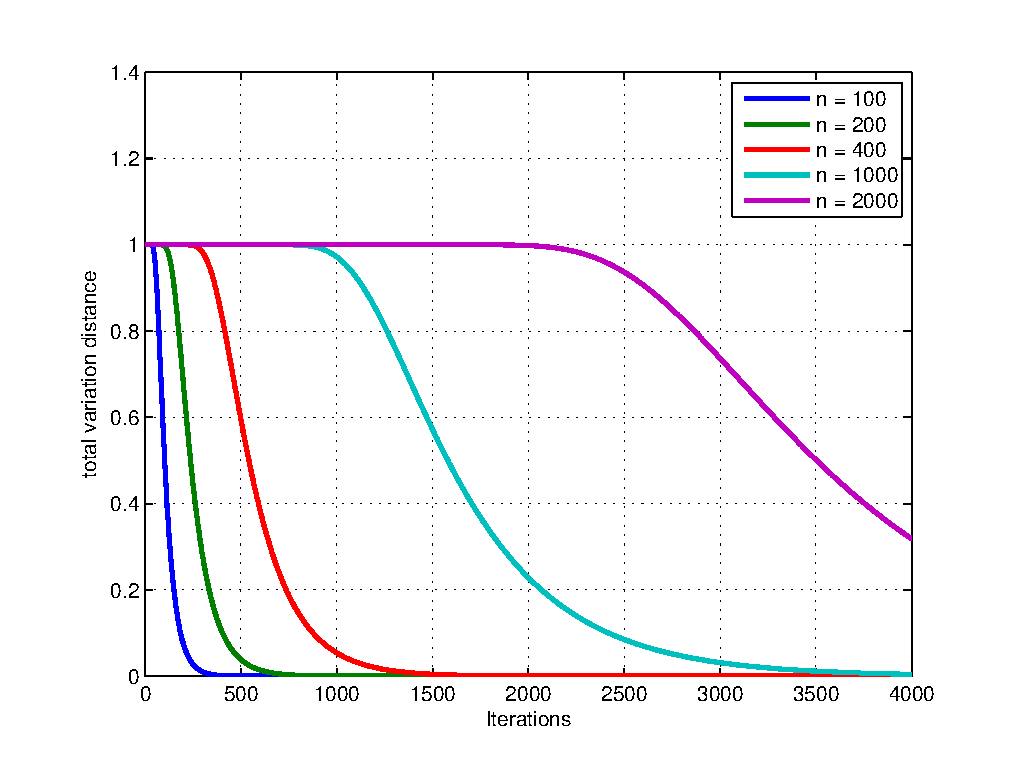
\includegraphics[width=0.7\textwidth,trim=1cm 1cm 0cm 0cm]{rdwalk}} \caption{The $k$
versus $|\omega_n^k-\bar{\omega}|_{TV}$ plot of random walk on an $n$-dimensional hypercube
problem. When $n$ increases, the distance stays close to $1$ for more iterations before it drops to
zero. }
\end{figure}

\end{example}

It is believed that cutoff phenomenon is widespread, although it has been proved only for a small
number of examples. The proof of cutoffs is in general very hard and varies case by case.


Although the study of cutoffs is focused on finite Markov Chains, we care more about what kind of
linear systems can generate convergence trajectories that have sharp changes. It is very hard
to image how a distribution would evolve abruptly to almost uniform from highly
concentrated (in a single state for finite Markov Chains). However, there is an excellent
explanation of why this happens. Consider another famous cutoff example: the Ehrenfest urn problem, involving $2$ urns and $n$
balls. In the beginning all the balls are in urn one, and at each iteration one of the balls is
chosen randomly and put in the other urn. This process is a Markov Chain and it can be shown that
this problem has the same total variation distance $|\omega^k_n-\bar{\omega}|_{TV}$ as the random
walk on hypercubes problem. In fact, this is how people analyze the random walk problem without
actually studying the $2^n$ system states. In this new Markov Chain, there are only $n+1$
states, which stand for the number of balls in urn $2$. In the beginning, all the balls are in urn
$1$ so the probability distribution is concentrated in the first state. The invariant distribution
of this reduced system is a binomial distribution centered at state $(n+1)/2$ (assuming $n$ is odd). By observing how the distribution is evolved when the system iterates, one would see two things:
first, the shape of the distribution gradually becomes binomial to fit the final shape; secondly,
the center of the distribution moves from $0$ toward $(n+1)/2$ at a certain speed (not a constant). When $n$ is large, not only does the center of the
distribution need more iterations to move to $(n+1)/2$, but also the shape of the distribution
needs more iterations to fit the stationary distribution. Cutoff is created by the combination of
these two effects. More details about this explanation can be found in \cite{Lloyd2005}. Now what decides the
shape of the cutoff when $n$ tends to infinity? When $n \to \infty$, a binomial distribution
can be well approximated by a normal distribution. Hence how the total variation distance changes near a
cutoff can be calculated by the TV of two normal distributions, and it has the
form like (\ref{rdwalkshape}). Therefore by forming the reduced system, we see clearly how a cutoff
can happen.





\paragraph{Chaotic Mixing.}
A widely observed phenomenon in the chaotic mixing process when small diffusion exists is the
two- or three-stage transition \cite{Thiffeault2003-13, Fereday2002, Antonsen1996}. The map
does not mix the scalar function with a constant rate in general. When the variance of the scalar
function is measured during the mixing process, one can in general observe a relatively flat decay
followed by a super-exponential change, and then finally it tends to an exponential decay. People
are interested in when these transitions happen, why they happen, and how to predict the slope of
the exponential region. A good review and physical interpretation can be found in
\cite{Thiffeault2004}.

In fact, such multi-stage mixing process can also be found in $1$-D chaotic map when a probability distribution is advected by the Perron-Frobenius operator of the map. To explain this, we first give the definition of the Perron-Frobenius operator \cite{Mezic2005}.

In the measure space $(X,\mathcal{A},\mu)$, for a map $S:X\to X$, we define the following operator. 
\begin{definition} \textbf{ (Perron-Frobenius operator)}
Let $\omega \in L^1(X)$, and suppose that for every $A \in \mathcal{A}$ the operator $P_S:L^1(X) \to L^1(X)$ satisfies
  \begin{eqnarray}
    \int_A P_S \omega(x)\mu(dx) = \int_{S^{-1}(A)} \omega(x)\mu(dx).
  \end{eqnarray}
Then $P_S$ is the Perron-Frobenius operator associated with $S$.
\end{definition}
It tells us how a probability distribution is evolved by a map $S$. 

%%%%%%%%%%%%%%%%%%%%%%%%%%%%%%%%%%%%%%%%%%%%%%
\begin{example} \textbf{Tent map cutoff.}
Consider the tent map
   \begin{eqnarray}
   \label{tentmap}
     x' = S_\text{tent}(x) = 1-2\left|x-\frac{1}{2}\right|
   \end{eqnarray}
with the following initial distributions on $[0 ,1]$:
  \begin{eqnarray}
  \label{tentmapinitial}
    \omega_n^0 = \begin{cases}
                      \frac{1}{\mu_n} &\text{ if } x \le \mu_n,\\
                      0               &\text{ otherwise},
                      \end{cases}
  \end{eqnarray}
where $\mu_1 = 1$, and $\mu_{n+1} = \mu_n/2$. The Perron-Frobenius operator of the tent map is
  \begin{eqnarray}
  \label{tentmapevolve}
    \omega_n^{k+1}(x) = P_\text{tent} \omega_n^{k}(x)
                             = \frac{1}{2}\left( \omega_n^{k}\left(\frac{x}{2}\right)+
                                                 \omega_n^{k}\left(1-\frac{x}{2}\right)  \right).
  \end{eqnarray}
The invariant distribution $\bar{\omega}$ of the tent map is uniform. Let $\nu_n^k =
|\omega_n^k-\bar{\omega} |_{TV}$; we find that
 \begin{eqnarray}
   \nu_n^k =  \begin{cases}
                    1- 2^{1+k-n}  &\text{ if }k \le n-1, \\
                    0             &\text{ otherwise}.
              \end{cases}
 \end{eqnarray}
The trajectories of $\nu_n^k$ with varying $n$ are shown in Figure \ref{tentmapcutoffplot}. It shows a cutoff.
\end{example}
%%%%%%%%%%%%%%%%%%%%%%%%%%%%%%%%%%%%%%%%%%%%%%%%
Hence we give the following simple theorem without proof.
%%%%%%%%%%%%%%%%%%%%%%%%%%%%%%%%%%%%%%%%%%%%%%%%
\begin{theorem} \textbf{(Tent map cutoff)}
\label{tentmapcutoff}
The family $(\Omega,\bar{\omega}, (\omega^k_n)_{k=0,1,\ldots})_{n=1,2,\ldots\,}$, where $\bar{\omega}$ is
uniform in $[0,1]$ and $\omega^k_n$ are defined as in (\ref{tentmapinitial}) and
(\ref{tentmapevolve}), presents a total variation-cutoff in the relaxed sense.
\end{theorem}
%%%%%%%%%%%%%%%%%%%%%%%%%%%%%%%%%%%%%%%%%%%%%%%%
A more general version of the above theorem and its proof can be found in section \ref{sec:mainresults}. Here we simply want to address that with the tent map and a sequence of suitable initial distributions, one can easily generate a sequence of Markov Chains that present a cutoff, though the shape is not normal.

This simple example shows that the tent map can present sharp changes in total variation distance. We would
like to generalize the result to a set of initial distributions and all $1$-D chaotic maps that have
full symbolic dynamics.



\begin{figure}
\centerline{{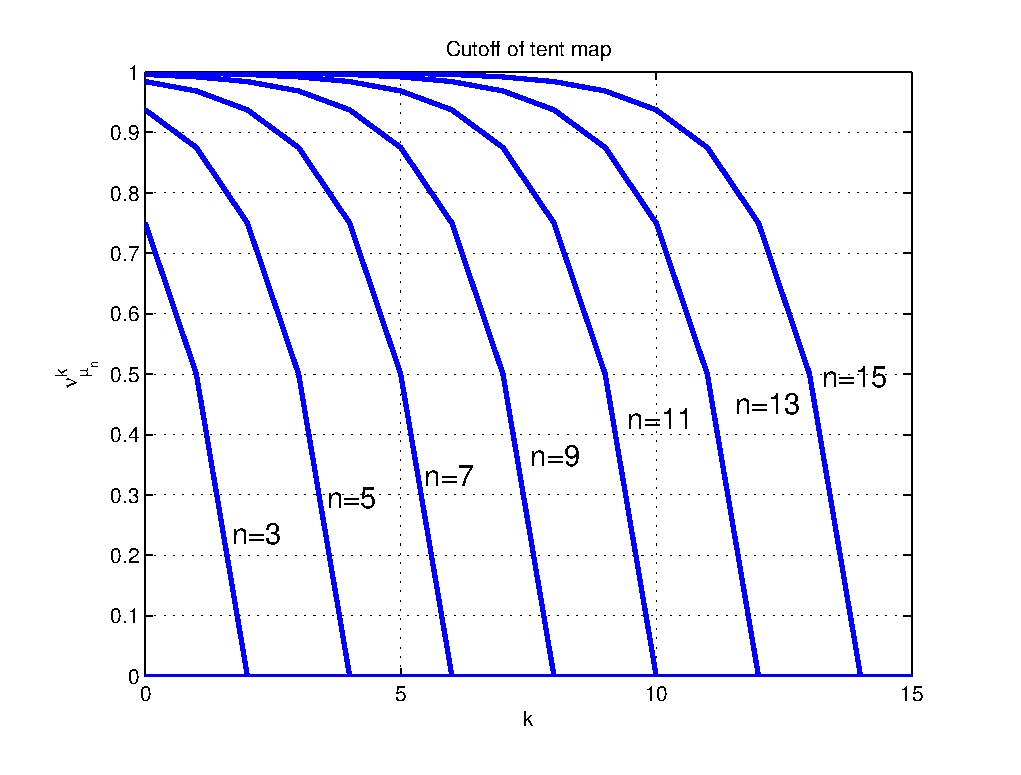
\includegraphics[width=0.7\textwidth]{tentmapcutoff.eps}}}
\caption{\label{tentmapcutoffplot} The plot of $\nu_n^k$. The trajectories present a cutoff.}
\end{figure}





%%%%%%%%
%%%%%%%%%%%%%%%%%%%%%%%%%%%%%%%%%%%%%%%%%%%%%%%%%%%%%%%%%%
%%%%%%%%%%%%%%%%%%%%%%%%%%%%%%%%%%%%%%%%%%%%%%%%%%%%%%%%%%
\section{Symbolic Dynamics and Stochastic Symbol Sequence}
\label{sec:symdyn}
%%%%%%%%%%%%%%%%%%%%%%%%%%%%%%%%%%%%%%%%%%%%%%%%%%%%%%%%%%
%%%%%%%%%%%%%%%%%%%%%%%%%%%%%%%%%%%%%%%%%%%%%%%%%%%%%%%%%%
%%%%%%%%%%%%%%%%%%%%%%%%%%%%%%
\subsection{Symbolic Dynamics}
%%%%%%%%%%%%%%%%%%%%%%%%%%%%%%
We briefly introduce symbolic dynamics for the study of chaotic maps. We focus on $1$-D chaotic maps, whose symbolic dynamics are semi-infinite sequences. 

Let $\mathcal{S}=\{L, R\}$ be the set of symbols consisting of $L$ and $R$. Define $\Sigma$, the collection of all semi-infinite sequence of elements of $\mathcal{S}$, i.e., $s\in \Sigma$ implies
 \begin{eqnarray}
 s= \{.s_0s_1\cdots s_n\cdots\}
 \end{eqnarray}
with $s_i\in \mathcal{S}$ for all $i$. We refer to $\Sigma$ as the space of semi-infinite sequence of two symbols. We consider a map $\sigma:\Sigma \to \Sigma$, which we shall call the shift map, defined as follows. For $s= \{.s_0s_1\cdots s_n\cdots\}$,
 \begin{eqnarray}
 \sigma(s)= \{.s_1s_2\cdots s_n\cdots\},
 \end{eqnarray}
i.e., the shift operator $\sigma$ simply deletes the first element of the sequence. There are rich results about the relation between symbolic dynamics and chaotic maps. Refer to \cite{Wiggins1990, Holmes1983} for good references. Roughly speaking, one can say that given a chaotic map $S$, on its invariant set $\Lambda$, the function $\phi(x): \Lambda \to \Sigma$, which maps a point in $x\in \Lambda$ to a semi-infinite sequence, is homeomorphism: $S$ acting on $\Lambda$ and $\sigma$ acting on $\Sigma$ are topologically conjugate. In other words, we have the following relation:
 \begin{eqnarray}
 S = \phi^{-1}\circ \sigma \circ \phi.
 \end{eqnarray}
And this explains the ``sensitive to initial condition'' property of chaotic maps.

All the results we derive in the next section in semi-infinite stochastic symbol sequences can be extended to bi-infinite ones without difficulty.

%Let $\mathcal{S}=\{L, R\}$ be the set of symbols consisting of $L$ and $R$. Let $\Sigma$ be the collection of all bi-infinite sequence of elements of $\mathcal{S}$, i.e., $s\in \Sigma$ implies
% \begin{eqnarray}
% s= \{\cdots s_{-n}\cdots s_{-1}.s_0s_1\cdots s_n\cdots\}
% \end{eqnarray}
%with $s_i\in \mathcal{S}$ for all $i$. We will refer to $\Sigma$ as the space of bi-infinite sequence of two symbols. We consider a map $\sigma:\Sigma \to \Sigma$, which we shall call the shift map, defined as follows: for $s= \{\cdots s_{-n}\cdots s_{-1}.s_0\cdots s_n\cdots\}$,
%  \begin{eqnarray}
% \sigma(s)= \{\cdots s_{-n}\cdots s_{-1}s_0.s_1\cdots s_n\cdots\}
% \end{eqnarray}
%$\sigma(\cdot)$ simply shift the dot one digit to the right of the sequence. There are rich results
%about the relation between symbolic dynamics and chaotic maps. Refer to \cite{Wiggins1990, Holmes1983} for good
%references. Roughly speaking, one can say that given a chaotic map $S$, on its invariant set
%$\Lambda$, the function $\phi(x): \Lambda \to \Sigma$, which maps a point in $x\in \Lambda$
%to a bi-infinite sequence, is homeomorphism: $S$ acting on $\Lambda$ and $\sigma$ acting on
%$\Sigma$ are topologically conjugate. In other words, we have the following relation,
% \begin{eqnarray}
% S = \phi^{-1}\circ \sigma \circ \phi
% \end{eqnarray}
%And this explains the ``sensitive to initial condition'' property of chaotic maps.

%In this paper we focus on the study of $1$-D chaotic maps, whose symbolic dynamics are semi-infinite sequences in stead of bi-infinite ones. 

%Define $\hat{\Sigma}$ the collection of all
%semi-infinite sequence of elements of $\mathcal{S}$. Each of the point $x \in \Lambda$ has $s\in
%\hat{\Sigma}$ with the following form,
% \begin{eqnarray}
% s= \{.s_0s_1\cdots s_n\cdots\}
% \end{eqnarray}
%The shift operator $\sigma$ simply deletes the first element of the sequence,
% \begin{eqnarray}
% \sigma(s)= \{.s_1s_2\cdots s_n\cdots\}
% \end{eqnarray}




%%%%%%%%%%%%%%%%%%%%%%%%%%%%%%%%%%%%%%%
\subsection{Stochastic Symbol Sequence}
%%%%%%%%%%%%%%%%%%%%%%%%%%%%%%%%%%%%%%%

Since our goal is to study how the probability density is evolved by the map, and symbolic dynamics
itself does not provide this information, we need a new object called stochastic symbol sequence.

%%%%%%%%%%%%%%%%%%%%%%%%%%%%%%%%%%%%%%%%%%%%%%%%%%%%%%%%%%%%%
% Definition
\begin{definition} \textbf{Stochastic symbol sequence.}
Consider $\mathcal{S}$ to be the symbol list. Let $\Delta$ be the collection of all
semi-infinite sequences of elements in $[0,1]$. We define $\delta^\star \in \Delta$ for each
symbol $\star \in \mathcal{S}$ as
 \begin{align}
 \begin{split}
 \delta^\star &= \{.\delta_0^\star \delta_1^\star\cdots \delta_n^\star\cdots\} \\
 %\delta^R &= \{\cdots \delta_{-n}^R\cdots \delta_{-1}^R.\delta_0^R \delta_1^R\cdots \delta_n^R\cdots\}
 \end{split} 
 \end{align}
with $\delta^\star_i \in [0,1]$ for all $i\ge 0$.
\end{definition}
%%%%%%%%%%%%%%%%%%%%%%%%%%%%%%%%%%%%%%%%%%%%%%%%%%%%%%%%%%%%%


The interpretation of each $\delta_i^\star$ is the probability of $x$ belonging to
symbol $\star$. Let $\Omega\in L^\infty[\Lambda], \int_\Lambda dz=1$ denote the space of
probability distribution in $\Lambda$. For a subspace  $\Lambda_\star \subset \Lambda$ and
$\omega\in \Omega$, we define $\psi^\star: \omega \mapsto \delta^\star$ as
 \begin{eqnarray}
 \label{psidef}
    %\delta^L_i = \int_{\Lambda_L} P^i_S \omega(z)dz \text{,   and  }
    \delta^\star_i = \int_{\Lambda_\star} P^i_S \omega(z)dz \text{, for all }i,
 \end{eqnarray}
where $P_S$ is the Perron-Frobenius operator of map $S$. Denote the $i$-th component of the symbolic dynamics of $x$ as $\phi(x)_i$. The above definition gives a simple relation between the symbolic dynamics and the stochastic symbol sequence. Suppose $x$ has pdf $\omega$, the stochastic symbol sequence of $\omega$ for symbol $\star \in \mathcal{S}$ is $\delta^\star$; then
 \begin{eqnarray}
 \label{deltaistar}
  \delta_i^\star = \prob(\phi(x)_i = \star) \text{, for } \star\in \mathcal{S} \text{ and all }i.
 \end{eqnarray} 

The definition is valid for any number of symbols. However, we only deal with two-symbol cases. For two-symbol cases: $\mathcal{S} = \{L,R\}$ and $\Lambda= \Lambda_L +\Lambda_R  $ , $\delta_i^R$ surely equals $1-\delta_i^L $. For simplicity, we
define $\psi = \psi^L$. We use $\delta$ to denote $\delta^L$ later. However, for clarity, we keep the $L$ for now. 


\begin{example} \textbf{Symbolic representation of the tent map}

Let $\Lambda=[0, 1]$. Partition $\Lambda \cap S^{-1}_{\text{tent}}(\Lambda)$ by writing its two
components as $\Lambda_L$ and $\Lambda_R$. For the tent map, $\Lambda_L=[0, 1/2]$ and $\Lambda_R=(1/2,1]$, we choose $\Lambda_R$ to exclude the point $1/2$ to avoid the overlap. We can associate with
each $x \in \Lambda $ a sequence $s = \{s_i \}_{i=0}^{\infty}$ of $L$'s and $R$'s defined by
$s_i=j$ if $S_{\text{tent}}^i(x) \in \Lambda_j$. The sequence ${s_i}$ labels the iterates of $x$
according to the left-right pattern they follow. In this way, we can label each $x \in \Lambda$
uniquely by a semi-infinite sequence $\phi(x)=s$ where the $s_i$'s are $L$'s and $R$'s. Let
$\Sigma$ denote the space of semi-infinite sequences of two symbols $L$'s and $R$'s. Then
$\phi(x): \Lambda \to \Sigma$ maps a point in $x\in I$ to a semi-infinite sequence.
The shift operator $\sigma$ acts on $s$ by simply dropping the first entry of $s$, i.e.,
$\sigma(\{s_i\}_{i=0}^{\infty})=\{s_i\}_{i=1}^{\infty}$. Similarly the map $\psi: \bar{\Omega}
\to \Delta$, where $\Delta$ denotes the space of semi-infinite stochastic
symbol sequence, maps an $\omega \in \bar{\Omega}$ to semi-infinite stochastic symbol sequences $\{
\delta^L,\delta^R\}$

%Note this is different from how it acts on a bi-infinity sequence, and this demonstrates that the
%tent map ``forgets'' the past information.
%An alternative interpretation of the semi-infinite
%sequence is as follows: one can embed the 1-D map into a 2-D volume preserved map, and make the
%symbol sequence bi-infinite. However, all the $s_i$'s with $i<0$ are unobservable. We can only
%evaluate (and we only care about) the thing happened in the first dimension.
\end{example}

It is clear that the map $\psi: \Omega \to \Delta $, as defined in
(\ref{psidef}), maps a probability distribution $\omega \in \Omega$ to the stochastic symbol
sequence $\delta$ uniquely. Moreover,  we overload the operator $\sigma$ to work
on the space $\Delta$, and have the following lemma.

%%%%%%%%%%%%%%%%%%%%%%%%%%%%%%%%%%%%%%%%%%%%%%%%%%%%%%%%%%%%%
%lemma
\begin{lemma}
  \begin{eqnarray}
 \psi \circ P_S = \sigma \circ \psi.
  \end{eqnarray}
\end{lemma}
\begin{proof} By definition,
  \begin{align}
      \delta_{i+1}^L (\omega)   &= \int_{\Lambda_L} P_S^{i+1} \omega(z)dz \nonumber\\
                                &= \int_{\Lambda_L} P_S^{i} \left(P_S\omega(z) \right) dz \nonumber\\
                                &=  \delta_{i}^L (P_S \omega).
  \end{align}
\end{proof}
%%%%%%%%%%%%%%%%%%%%%%%%%%%%%%%%%%%%%%%%%%%%%%%%%%%%%%%%%%%%%

However, unlike $\phi$, the function $\psi$ is not invertible. There are many $\omega$'s that map to the same $\delta^L$. To resolve this problem, for a given chaotic map $S$ we consider a smaller space:
  \begin{eqnarray}
  \label{DefOmegabar}
  \bar{\Omega} = \left\{ \omega \mid \omega(z) = \lim_{n \to \infty} \prod_{i=0}^n \beta^{\phi(z)_i}_i \right\},
  \end{eqnarray}
where $\beta^L_i \in [0,1]$, $\beta^R_i=1-\beta^L_i$. Remember that $\phi(z)_i$ is the $i$-th component of the symbol sequence of $z$ associated with the chaotic map, so having symbolic dynamics is a necessary condition for having $\bar{\Omega}$.

%%%%%%%%%%%%%%%%%%%%%%%%%%%%%%%%%%%%%%%%%%%%%%%%%%%%%%%%%%%%%
The following lemma justifies the existence of $\psi^{-1}$ in $\bar{\Omega}$.
%lemma
\begin{lemma} For $\omega \in \bar{\Omega}$, one has
 \begin{eqnarray}
    \delta^L_k(\omega) = \beta^L_k(\omega)  \text{, for all }k.
 \end{eqnarray}
\end{lemma}
\begin{proof} By definition,
 \begin{align}
    \delta_{k}^L (\omega)   &= \int_{\Lambda_L} P_S^{k} \omega(z)dz \nonumber\\
                            &= \int_{S^{-k}(\Lambda_L)} \omega(z)dz \nonumber\\
                            &= \lim_{n \to \infty} \sum_{\substack{s\in \Sigma\\s^k= L }}  \prod_{i=0}^{n} \beta^{s_i}_i \nonumber\\
                            &= \beta_k^L \lim_{n \to \infty} \sum_{s\in \Sigma}  \prod_{\substack{i=0\\ i\neq k}}^{n} \beta^{s_i}_i \nonumber\\
                            &= \beta_k^L.
 \end{align}
\end{proof}
%%%%%%%%%%%%%%%%%%%%%%%%%%%%%%%%%%%%%%%%%%%%%%%%%%%%%%%%%%%%%

Hence, in $\bar{\Omega}$ the map $\psi$ is invertible. From now on, the probability space we are interested in is the space $\bar{\Omega}$. It is also easy to check that
 \begin{eqnarray}
 \label{Pconserve}
  P_S (\omega) \in \bar{\Omega}, \mbox{ if } \omega \in \bar{\Omega}.
 \end{eqnarray}
And since $\psi$ is invertible, just like in symbolic dynamics, we also have
 \begin{eqnarray}
 P_S= \psi^{-1}\circ \sigma \circ \psi.
 \end{eqnarray}
It says the Perron-Frobenius operator and the shift operator are conjugate in the spaces $\{\bar{\Omega},\Delta \}$. To understand the special property of the subspace $\bar{\Omega}$, we give the following lemma.

%%%%%%%%%%%%%%%%%%%%%%%%%%%%%%%%%%%%%%%%%%%%%%%%%%%%%%%%%%%%%
%lemma
\begin{lemma} \label{lemma:independency}
For $x \in \Lambda$ having pdf $\omega \in \bar{\Omega}$, and any $s\in \Sigma$, then for any $i,j$, $i\neq j$, 
\begin{equation}
   \phi(x)_i=s_i \mbox{ and } \phi(x)_j=s_j \mbox{ are independent.}
\end{equation}
\end{lemma}
\todo{TC: there might be a better way to state the independence, and need to check is the proof strong enough.}
%one has
% \begin{equation}
%    \prob(\phi(x)_i=s_i) =   \prob(\phi(x)_i=s_i \mid  \phi(x)_k=s_k, k= {0,\ldots,\infty\}, k \neq i )
% \end{equation}
%\end{lemma}

\begin{proof} For $\omega\in \bar{\Omega}$, 
 \begin{align*}
   \prob(\phi(x)=s) &= \lim_{n \to \infty} \prod_{i=0}^{n} \delta_i^{s_i}  \\
                      &=  \lim_{n \to \infty} \prod_{i=0}^{n} \prob(\phi(x)_i=s_i).
 \end{align*}
The second equality is from equation (\ref{deltaistar}). This justifies the claim of independence.   
\end{proof}
%%%%%%%%%%%%%%%%%%%%%%%%%%%%%%%%%%%%%%%%%%%%%%%%%%%%%%%%%%%%%


Furthermore, we define the convex combination of two stochastic symbol sequences to be the convex combination of the individual components and then give another important property of the function $\psi$.
%%%%%%%%%%%%%%%%%%%%%%%%%%%%%%%%%%%%%%%%%%%%%%%%%%%%%%%%%%%%%
%lemma
\begin{lemma}
For any $\omega_1, \omega_2 \in \bar{\Omega}$ and $\alpha\in[0,1]$, one has
 \begin{eqnarray}
 \label{psiislinear}
  \psi(\alpha\omega_1+(1-\alpha)\omega_2) = \alpha\psi(\omega_1)+(1-\alpha)\psi(\omega_2).
 \end{eqnarray}
\end{lemma}

\begin{proof}
  \begin{align}
    \lefteqn{\alpha \delta^L_k(\omega_1) + (1-\alpha) \delta^L_k(\omega_2) } \nonumber\\
                    &=   \alpha \int_{S^{-k}(\Lambda_L)} \omega_1(z)dz+
                          (1-\alpha) \int_{S^{-k}(\Lambda_L)} \omega_2(z)dz \nonumber \\
                    &=   \int_{S^{-k}(\Lambda_L)}\left( \alpha \omega_1(z) +(1-\alpha) \omega_2(z) \right) dz \nonumber \\
                    &=   \delta^L_k( \alpha \omega_1 +(1-\alpha) \omega_2).
  \end{align}
\end{proof}
%%%%%%%%%%%%%%%%%%%%%%%%%%%%%%%%%%%%%%%%%%%%%%%%%%%%%%%%%%%%%
 This property can be extended to the convex combination of $n$ distributions and allows us to prove some important facts later.


We have successfully moved from the probability distribution $\omega \in \bar{\Omega}$ to its
stochastic symbol sequence representation. Now we would like to know how total variation distance
passes through, i.e., given $\omega$ and $\bar{\omega}$ with stochastic symbol sequence
$\{\delta^L, \delta^R\}$ and $\{\bar{\delta}^L,\bar{\delta}^R \}$, respectively, how do we calculate
$|\omega-\bar{\omega}|_{TV}$? The answer is:
 \begin{eqnarray}
 \label{infiniteTV}
|\omega-\bar{\omega}|_{TV} = \frac{1}{2} \lim_{n \to \infty}  \sum_{s\in\Sigma} \left| \prod_{i=0}^n\delta_i^{s_i}-\prod_{i=0}^n\bar{\delta}_i^{s_i}  \right|.
 \end{eqnarray}
This expression is almost impossible to evaluate because of the summation over infinity combinations. So let us consider a simpler case, when $\delta^L$ and $\bar{\delta}^L$ only have $p$ different digits, i.e.,\ $\delta_i^L = \bar{\delta}_i^L$ when $i\notin \theta$, and $|\theta| = p$. Let $\Sigma_p$ be the space of all combinations of $p$ symbol sequence with two symbols. Then we have
 \begin{eqnarray}
  \label{finiteTV}
|\omega-\bar{\omega}|_{TV} = \frac{1}{2} \sum_{s\in\Sigma_p}  \left| \prod_{i\in \theta}\delta_i^{s_i}-\prod_{i\in\theta}\bar{\delta}_i^{s_i}  \right|.
 \end{eqnarray}
In this expression, $s$ is some finite selections of the bi-infinite symbol sequence. The message here is that the total variation distance has nothing to do with the order: it only depends on the elements $s_i, i\in\theta$. Furthermore, (\ref{finiteTV})  can serve as a lower bound when the information besides $i\in \theta$ is unknown.







%%%%%%%%%%%%%%%%%%%%%%%%%%%%%%%%%%%%%%%%%%%%%%%%%%%%%%%%%%
\subsection{General results}
In reality, we may not care about the TV between two probability distributions, but want to know which one of them is closer to the invariant measure of the map. In this section, we give some general results about the TV from a stochastic symbol sequence of two symbols to the distribution $\bar{\omega}$, which has the representation
\begin{equation}
\label{deltabar}
\bar{\delta}=\left\{.\frac{1}{2}\frac{1}{2}\frac{1}{2}\cdots\right\}.
\end{equation}
Clearly (\ref{deltabar}) is invariant under the shift operator, and hence it is an invariant measure of the map. From now on we use $\delta$ to denote $\delta^L$, and if needed, $1-\delta$ represents $\delta^R$. Also, $\delta$ itself without any sub-index represents the whole stochastic symbol sequence, and $\delta_i$ indicates the $i$-th component in $\delta$ on the right-hand side of the dot.

\todo{TC:(\ref{deltabar}) is not the only invariant measure. Any constant sequence is invariant under the shift map, but we are not interested in them.}

The following convexity lemma is the basis of all later results.
%%%%%%%%%%%%%%%%%%%%%%%%%%%%%%%%%%%%%%%%%%%%%%%%%%%%%%%%%%%%%
%lemma
\begin{lemma} For $\delta,\delta^* \in \Delta$, $\alpha\in [0 ,1]$,
 \begin{eqnarray}
\label{convexityofTV}
|\psi^{-1}(\alpha\delta+(1-\alpha)\delta^*)-\bar{\omega}|_{TV} \le
            \alpha|\psi^{-1}(\delta)-\bar{\omega} |_{TV}+(1-\alpha)|\psi^{-1}(\delta^*)-\bar{\omega}|_{TV}.
 \end{eqnarray}
\end{lemma}
\begin{proof}
Since $\omega \mapsto |\omega-\bar{\omega}|_{TV}$ is a convex function, by using
(\ref{psiislinear}) we obtain that the function $\delta \mapsto
|\psi^{-1}(\delta)-\bar{\omega}|_{TV} $ is also convex. The convexity gives us the above
result.
\end{proof}
%%%%%%%%%%%%%%%%%%%%%%%%%%%%%%%%%%%%%%%%%%%%%%%%%%%%%%%%%%%%%



So even if there is no direct way to calculate the TV from a stochastic symbol
sequence to another, we can still use the convexity to deduce some useful bounds.

We give the following lemmas.

%%%%%%%%%%%%%%%%%%%%%%%%%%%%%%%%%%%%%%%%%%%%%%%%%%%%%%%%%%%%%
%lemma
\begin{lemma}
\label{onedifflemma} Suppose $\delta$ and $\delta^*$ are two stochastic symbol sequences corresponding
to the probability distribution $\omega$ and $\omega^*$, respectively. Suppose there exists a
bijection $\gamma: i \mapsto j$ such that $\delta_i = \delta^*_j$ for all $i\in
\mathbb{Z}\setminus\{i^\dagger\}$. If $ |\delta_{i^\dagger}-\frac{1}{2}| \ge |\delta^*_{\gamma(i^\dagger)}-\frac{1}{2}|$, then
 \begin{eqnarray}
      |\omega-\bar{\omega} |_{TV} \ge |\omega^*-\bar{\omega} |_{TV}.
 \end{eqnarray}
\end{lemma}
\begin{proof} Since $|\psi^{-1}(\delta)-\bar{\omega}|_{TV}$ is independent of the order of the sequence, we can assume
$\delta = \delta^*$ for all $i\in \mathbb{Z}\setminus\{i^\dagger\}$. Let $\tilde{\delta} = \delta$
for all $i\in \mathbb{Z}\setminus\{i^\dagger\}$, and
$\tilde{\delta}_{i^\dagger}=1-\delta_{i^\dagger}$. Apparently,
$|\psi^{-1}(\delta)-\bar{\omega}|_{TV} =|\psi^{-1}(\tilde{\delta})-\bar{\omega}|_{TV} $. When
$|\delta_{i^\dagger}-\frac{1}{2}| \ge |\delta^*_{i^\dagger}-\frac{1}{2}|$, it is always possible to
choose $\alpha\in[0,1]$ such that  $\delta^*_i = \alpha \delta_i +(1-\alpha) \tilde{\delta}_i $.
Applying (\ref{convexityofTV}) to $\delta$ and $\tilde{\delta}$ with the $\alpha$ above, we have
\begin{align}
    |\psi^{-1}(\delta^*)-\bar{\omega}|_{TV}
                 &\le  \alpha|\psi^{-1}(\delta)-\bar{\omega} |_{TV}+(1-\alpha)|\psi^{-1}(\tilde{\delta})-\bar{\omega}|_{TV} \nonumber\\
                 & =  |\psi^{-1}(\delta)-\bar{\omega} |_{TV}.
 \end{align}
\end{proof}
%%%%%%%%%%%%%%%%%%%%%%%%%%%%%%%%%%%%%%%%%%%%%%%%%%%%%%%%%%%%%

%%%%%%%%%%%%%%%%%%%%%%%%%%%%%%%%%%%%%%%%%%%%%%%%%%%%%%%%%%%%%
%lemma
\begin{lemma}
\label{alldifflemma} Suppose $\delta$ and $\delta^*$ are two stochastic symbol sequences corresponding
to the probability distribution $\omega$ and $\omega^*$, respectively. Suppose there exists a
bijection $\gamma: i \mapsto j$ such that $|\delta_i-\frac{1}{2}| \ge |\delta^*_j-\frac{1}{2} |$ for
all $i\in \mathbb{Z}$. Then
 \begin{eqnarray}
   |\omega-\bar{\omega} |_{TV} \ge|\omega^*-\bar{\omega} |_{TV}.
 \end{eqnarray}
\end{lemma}
\begin{proof} Apply Lemma \ref{onedifflemma} repeatedly.
\end{proof}
%%%%%%%%%%%%%%%%%%%%%%%%%%%%%%%%%%%%%%%%%%%%%%%%%%%%%%%%%%%%%

The above lemma tells us how to compare $|\omega-\bar{\omega}|_{TV}$ and $|\omega^*-\bar{\omega}|_{TV}$
if some relation of their stochastic symbol sequences is known. Now for a given $\omega$ we want
to bound its $|\omega-\bar{\omega}|_{TV}$ by choosing an $\omega^*$ such that its
$|\omega^*-\bar{\omega}|_{TV}$ is easy to calculate. The choices we made are the sequences with the
following form:
  \begin{align}
  \begin{split}
  \label{deltamM}
   \delta^m &= \{.\underbrace{\delta^m_{\star} \delta^m_{\star} \cdots \delta^m_{\star}}_{p}\frac{1}{2}\frac{1}{2}\cdots \}, \\
   \delta^M &= \{.\underbrace{\delta^M_{\star} \delta^M_{\star} \cdots \delta^M_{\star}}_{p}\frac{1}{2}\frac{1}{2}\cdots \}.
  \end{split}
  \end{align}
As we see later, $|\omega-\bar{\omega}|_{TV}$ can be evaluated easily if $\psi^{-1}(\omega)$ has finite constant leading terms. Note that we use the index $\star$ to indicate that $\delta_{\star}^M$ and $\delta_{\star}^m$ are numbers, not sequences.

  
%Where $\delta^m_0=\delta^m_1= \cdots = \delta^m_{p-1} \equiv \delta^m_{\star}$ and
%$\delta^M_0=\delta^M_1= \cdots = \delta^M_{p-1}\equiv \delta^M_{\star}$.


%First we are going to generalize the lower bound result from $\delta_i=1$, for $i\in \theta$ to $\delta_i=\delta^M$. Note here $\delta^M$ is a number, $1/2 \le \delta^M \le 1$.

%%%%%%%%%%%%%%%%%%%%%%%%%%%%
\subsubsection{Lower Bound}
%%%%%%%%%%%%%%%%%%%%%%%%%%%%%

%%%%%%%%%%%%%%%%%%%%%%%%%%%%%%%%%%%%%%%%%%%%%%%%%%%%%%%%%%%%%
%theorem
\begin{theorem}
\label{theoremlb} Suppose $\delta$ and $\bar{\delta}$ are two stochastic symbol sequences corresponding
to the probability distribution $\omega$ and the invariant distribution $\bar{\omega}$,
respectively. Suppose there is a set $\theta \subset \mathbb{Z}^++\{0\} $, $|\theta|=p$ such that
for all $i \in \theta$, $|\delta_i-\frac{1}{2}|>|\delta^m_\star-\frac{1}{2}|$. Then
\begin{eqnarray}
\label{lbineq}
|\omega-\bar{\omega}|_{TV} \ge \mathbf{I}_{\frac{1}{2}}(p-q^*,q^*+1) - \mathbf{I}_{1-\delta^m_\star}(p-q^*,q^*+1),
\end{eqnarray}
where
\begin{eqnarray}
\label{kstar}
q^* =  \left\lfloor p \frac{\log{2}+\log{(\frac{1}{2}-\epsilon)} }{\log{(\frac{1}{2}-\epsilon)}-\log{(\frac{1}{2}+\epsilon})} \right\rfloor,
\end{eqnarray}
$\epsilon = |\delta^m_\star-\frac{1}{2}|$, and $\mathbf{I}$ is the regularized incomplete
beta function.
\end{theorem}
\begin{proof}
Since the TV is independent of the order of the sequence, we can assume that
$\theta=\{0,1,\ldots,p-1\}$. Also, without loss of generality, we assume for $i\in \theta$,
$\delta_i \ge \epsilon+\frac{1}{2}= \delta^m_\star$. Using equation (\ref{finiteTV}) and Lemma
\ref{alldifflemma}, we have
\begin{align}
\label{lbtv}
|\omega-\bar{\omega}|_{TV}
                      &\ge \frac{1}{2} \sum_{s\in\Sigma_p}
                             \left| \prod_{i\in \theta}\delta_i^{s_i}-\prod_{i\in\theta}\bar{\delta}_i^{s_i}  \right| \nonumber\\
                      &\ge \frac{1}{2}  \sum_{q=0}^{p}
                             {p \choose q} \left|(\delta^m_\star)^q (1-\delta^m_\star)^{p-q} - \frac{1}{2^p} \right| \nonumber \\
                      &=   \frac{1}{2}  \sum_{q=0}^{p} \left|{p \choose q} (\delta^m_\star)^q (1-\delta^m_\star)^{p-q} -{p \choose q} \frac{1}{2^p} \right|.
\end{align}
\end{proof}
\todo{TC: The first line is an inequality because $p < \infty$. }

%%%%%%%%%%%%%%%%%%%%%%%%%%%%%%%%%%%%%%%%%%%%%%%%%%%%%%%%%%%%%

So the total variation distance can be lower bounded by the difference between two binomial
distributions. We can find their difference by subtracting their cumulative distribution functions
at the point they cross over each other. To do this we needs to find the point where the first
distribution begins to exceed the second distribution, which is to find the largest $q^*$ such that
\begin{eqnarray}
\left(\frac{1}{2}+\epsilon\right)^{q^*}\left(\frac{1}{2}-\epsilon\right)^{p-1-q^*}-2^{-p} \le 0.
\end{eqnarray}
Solving for $q^*$ gives (\ref{kstar}), and the cdf of a binomial distribution can be expressed in terms
of the regularized incomplete beta function $\mathbf{I}$ as follows. For the distribution
$\text{binomial}(r,p)$, its cdf is
\begin{eqnarray}
   F(q;p,r) = \mathbf{I}_{1-r}(p-q,q+1).
\end{eqnarray}
Substituting $q^*$ into $q$, and $1/2$ and $\delta^m_\star$ into $r$, we get (\ref{lbineq}).
%\begin{eqnarray}
%|\omega-\bar{\omega}|_{TV} \ge \mathbf{I}_{\frac{1}{2}}(p-k^*,k^*+1) - \mathbf{I}_{1-\delta^m}(p-k^*,k^*+1)
%\end{eqnarray}


An interesting corollary is that when $p$ goes to $\infty$, $|\omega-\bar{\omega}|_{TV}$ goes
to $1$ for all $\epsilon>0$. So each of the constant stochastic symbol sequences actually
represents an eigenfunction or an invariant measure of the map with eigenvalue $1$.




%%%%%%%%%%%%%%%%%%%%%%%%%%%
\subsubsection{Upper Bound}
%%%%%%%%%%%%%%%%%%%%%%%%%%%

We have seen that for a constant sequence with components not equal to $1/2$, the total variation
distance to the invariant distribution $\bar{\omega}$ is $1$ from the previous theorem. Hence this
result does not give us any information about the upper bound. We would like to bound the distance
by the sum of the sequence, and give the following theorem.
\begin{theorem}
\label{theoremub}Suppose $\delta$ and $\bar{\delta}$ are two stochastic symbol sequences corresponding
to the probability distribution $\omega$ and the invariant distribution $\bar{\omega}$,
respectively. Suppose $\sum_{i=0}^\infty |\delta_i - \frac{1}{2}| = \frac{M}{2}$. Then
\begin{eqnarray}
|\omega-\bar{\omega}|_{TV} \le  \begin{cases}
                                   \rho - 2^{-\lceil M \rceil } &\text{ if } \rho>1-2^{-\lceil M \rceil },\\
                                    1-2^{-\lfloor M \rfloor}    &\text{ otherwise},                                   \\
                                \end{cases} 
\end{eqnarray}
where $\rho = \frac{1}{2} +  \frac{M-\lfloor M \rfloor}{2}$.
\end{theorem}
\begin{proof}
With the convexity inequality (\ref{convexityofTV}), one can show that for a set of stochastic symbol sequence $\delta^j$, $j=\{1,2,\ldots\}$, $\sum_j{\alpha_j} = 1$,
\begin{eqnarray}
 \sum_j \alpha_j|\psi^{-1}(\delta^j)-\bar{\omega}|_{TV} \ge |\psi^{-1}(\sum_j \alpha_j \delta^j)-\bar{\omega}|_{TV}.
\end{eqnarray}
So for each $M$, if we can express $\delta$ as the convex combination of a set of $\delta^j$, the total variation distance $|\omega-\bar{\omega}|_{TV}$ can be bounded by the TV of individual $\delta^j$. Let the set $\mathbf{C} = \{\delta \, | \,\sum_i|\delta_i-\frac{1}{2}|  =  \frac{M}{2}\}$. It is easy to see that $\mathbf{C} = \mathbf{conv} \mathbf{D}$, where $\mathbf{D}$ is defined as
\begin{eqnarray}
  \mathbf{D}=\{\delta \mid \delta \text{ has } \lfloor M \rfloor \text{ } 1\text{'s, one } M-\lfloor M \rfloor
               \text{, and all other }\delta_i\text{'s are }\frac{1}{2}  \},
\end{eqnarray}
and $|\psi^{-1}(\delta)-\bar{\omega}(x)|_{TV}$ for each $\delta \in  \mathbf{D}$ can be calculated as
\begin{eqnarray}
|\psi^{-1}(\delta)-\bar{\omega}(x)|_{TV} = 
          \begin{cases}
             \rho - 2^{-\lceil M \rceil } &\text{ if } \rho>1-2^{-\lceil M \rceil },\\
             1-2^{-\lfloor M \rfloor}    &\text{ otherwise},                                   
          \end{cases}
\end{eqnarray}
where $\rho = \frac{1}{2} +  \frac{M-\lfloor M \rfloor}{2}$. We obtain the upper bound by choosing the set of $\delta^j$ to be $\mathbf{D}$.
\end{proof}

Unfortunately, the above upper bound is in general not very tight. We state it just to inspire the next theorem, which gives a tighter bound.
%%%%%%%%%%%%%%%%%%%%%%%%%%%%%%%%%%%%%%%%%%%%%%%%%%%%%%%%%%%%%%%%%%%%%%%%%%%%%%%%%%%%%%%%

\begin{theorem}
\label{theoremub2}
Suppose $\delta$ and $\bar{\delta}$ are two stochastic symbol sequences corresponding to the probability distribution $\omega$ and the invariant distribution $\bar{\omega}$, respectively. Suppose $\sum_{i=0}^\infty |\delta_i - \frac{1}{2}| = \frac{M}{2}$, and $\delta_i \le \delta^M_\star$ for all $i$. Then
\begin{eqnarray}
\label{ubineq}
|\omega-\bar{\omega}|_{TV} \le  \mathbf{I}_{\frac{1}{2}}(p-q^*,q^*+1) - \mathbf{I}_{1-\delta^M_\star}(p-q^*,q^*+1)
\end{eqnarray}
with
\begin{eqnarray}
\label{kstarub}
q^* =  \left\lfloor p \frac{\log{2}+\log{(\frac{1}{2}-\epsilon)} }{\log{(\frac{1}{2}-\epsilon)}-\log{(\frac{1}{2}+\epsilon})}  \right\rfloor,
\end{eqnarray}
where $\epsilon = |\delta^M_\star - \frac{1}{2}|$ and $p = \lceil \frac{M}{2\epsilon}\ \rceil$.
\end{theorem}

\begin{proof} Similarly to the previous proof, let
\begin{eqnarray}
  \mathbf{D}=\{\delta \mid \delta \text{ has } (p-1)\text{ }  of \text{ } \delta^M_\star\text{'s, one } M-(p-1) \delta^M_\star
                \text{, and all other }\delta_i\text{'s are }\frac{1}{2}   \}.
\end{eqnarray}
Then the set  $\mathbf{C} = \{\delta \mid \sum_i|\delta_i-\frac{1}{2}|  =  \frac{M}{2}\}$ satisfies $\mathbf{C} = \mathbf{conv} \mathbf{D}$. All $\delta \in \mathbf{D}$ have the same $|\psi^{-1}(\delta) - \bar{\omega}|_{TV} $ and are bounded by
\begin{eqnarray}
\label{middleineq}
 |\psi^{-1}(\delta) - \bar{\omega}|_{TV} < |\psi^{-1}(\delta^M) - \bar{\omega}|_{TV},
\end{eqnarray}
and $|\psi^{-1}(\delta^M) - \bar{\omega}|_{TV}$ can be calculated similarly to the lower bound proof by finding the $q^*$ such that the first binomial distribution is less than the second one, i.e., find the smallest $q^*$ such that
\begin{eqnarray}
\left(\frac{1}{2}+\epsilon\right)^{q^*}\left(\frac{1}{2}-\epsilon\right)^{p-q^*}-2^{-p} \ge 0.
\end{eqnarray}
Once $q^*$ is solved as in (\ref{kstarub}), we have $|\psi^{-1}(\delta^M) - \bar{\omega}|_{TV} = \mathbf{I}_{\frac{1}{2}}(p-q^*,q^*+1) - \mathbf{I}_{1-\delta^M_\star}(p-q^*,q^*+1)$. Combining with (\ref{middleineq}), one gets (\ref{ubineq}).
\end{proof}



%%%%%%%%%%%%%%%%%%%%%%%%%%%%%%%%%%%%%%%%%
% approximated lower and upper bound
%%%%%%%%%%%%%%%%%%%%%%%%%%%%%%%%%%%%%%%%%
The above lower and upper bound theorems can be applied to any given stochastic symbol sequence as long as one can find $\delta^m$ and $\delta^M$ to bound it. In the following theorem, we consider a scenario that $p \to \infty$ and
$\delta^m_\star (\text{or } \delta^M_\star)\to 1/2$ and calculate where the lower and upper bounds converges to.

%%%%%%%%%%%%%%%%%%%%%%%%%%%%%%%%%%%%%%%%%%%%%%%%%%%%%%%%%
\begin{theorem}
\label{theoremapproxlb} Suppose $\bar{\omega}$ and $\omega_{lb}$ (resp.\ $\omega_{ub}$) are two probability distributions with stochastic symbol sequences $\bar{\delta}$ and $\delta^m$ (resp.\ $\delta^M$) as defined in (\ref{deltabar}) and (\ref{deltamM}), respectively. If $p
\to \infty$ and $\delta^m_{\star}$ (resp.\ $\delta^M_{\star}$)$ \to \frac{1}{2}$, then one has
\begin{align}
\begin{split}
  \label{lbublimit}
                 |\omega_{lb}-\bar{\omega}|_{TV}
               & =  \erf \left( \sqrt{\frac{p}{2}}\left((\delta_{\star}^m)-\frac{1}{2}\right)\right), \\
  \text{resp. }  |\omega_{ub}-\bar{\omega}|_{TV}
               & =  \erf \left( \sqrt{\frac{p}{2}}\left((\delta_{\star}^M)-\frac{1}{2}\right)\right).
\end{split}
\end{align}


\end{theorem}
\begin{proof}
When $p\to \infty$ the binomial distribution approaches the normal distribution as $\text{binomial}\ (\delta^m_{\star},p) \to \mathcal{N}(p\delta^m_{\star}, p\delta^m_{\star}(1-\delta^m_{\star}))$.  The term $|\omega_{lb}-\bar{\omega}|_{TV}$ thus equals the TV between two normal distributions, which can be evaluated by subtracting their cdfs: %Let $(\omega^m)^k \equiv \psi^{-1}(\sigma^k(\delta^M)) $
\begin{align}
  |\omega_{lb}-\bar{\omega}|_{TV}
              &=  \frac{1}{2}\left(1+\erf\left(\frac{x^*-p\delta_{\star}^m}{\sqrt{2p\delta_{\star}^m(1-\delta_{\star}^m)}}\right)\right)
                       -\frac{1}{2}\left(1+\erf\left(\frac{x^*-p\frac{1}{2}}{\sqrt{2p\frac{1}{2}(1-\frac{1}{2})}}\right)\right) \nonumber\\
              &=\erf\left(\frac{x^*-p\delta_{\star}^m}{\sqrt{2p\delta_{\star}^m(1-\delta_{\star}^m)}}\right)-
                       \erf\left(\frac{x^*-p\frac{1}{2}}{\sqrt{2p\frac{1}{2}(1-\frac{1}{2})}}\right),
\end{align}
where $x^*$ is the point the two pdfs crosses over each other. When $\delta_{\star}^m \to \frac{1}{2}$, the denominators in both
$\erf(\cdot)$ are the same, and hence the variances of the two normal distributions are the same while the means differ by
$p(\delta^m_{\star}-\frac{1}{2})$, and one gets (\ref{lbublimit}). Same for the $\omega_{ub}$ equality.

\end{proof}




%Just like the lower bound, we can also give an approximate upper bound,
%\begin{theorem}
%\label{theoremapproxub}  $\delta$ and $\bar{\delta}$ are two stochastic symbol sequences, each
%corresponds to the probability distribution $\omega$ and the invariant distribution $\bar{\omega}$,
%respectively. Suppose $\sum_{i=0}^\infty |\delta_i - \frac{1}{2}| = \frac{M}{2}$, and $p$ is large
%and $\delta^M_\star$ close to $\frac{1}{2}$, then
%\begin{eqnarray}
%\label{lbineqapprox}
%    |\omega-\bar{\omega}|_{TV}   \le  \erf\left( \sqrt{p}\left((\delta_{\star}^M)-\frac{1}{2}\right)\right)
%\end{eqnarray}


%\end{theorem}
%\paragraph{proof} Similar to theorem \ref{theoremapproxlb}




%%%%%%%%%%%%%%%%%%%%%%%%%%%%%%%%%%%%%%%%%%%%%%%%%%%%%%%%%%
%%%%%%%%%%%%%%%%%%%%%%%%%%%%%%%%%%%%%%%%%%%%%%%%%%%%%%%%%%
\section{Main results}
\label{sec:mainresults}
%%%%%%%%%%%%%%%%%%%%%%%%%%%%%%%%%%%%%%%%%%%%%%%%%%%%%%%%%%
%%%%%%%%%%%%%%%%%%%%%%%%%%%%%%%%%%%%%%%%%%%%%%%%%%%%%%%%%%
In the previous section we only deal with the relation between given $\omega$ and $\bar{\omega}$, and there is no evolution. In this section we talk about how to use the results we have to bound $|\omega^k-\bar{\omega}|_{TV}$ when the system iterates with $k$. In general it is no easier to find the stochastic symbol sequence of a probability distribution than to evolve it by the chaotic map directly. Therefore the upper and lower bounds are not practically applicable to tell us the shape of the convergence trajectory for a given initial distribution. Nonetheless, they do provide us a way to observe what creates the sharp change in the total variation distances: the moving and reshaping of a binomial (or binomial-like) distribution to another. Here we consider two interesting examples, where given the stochastic symbol sequences of some functions, we can observe how their $|\omega^k-\bar{\omega}|_{TV}$ change.

\begin{example}
\label{example:constantoega0}
Suppose $\omega^0$ has stochastic symbol sequence as follows:
  \begin{eqnarray}
  \label{constantomega0}
   \psi(\omega^0) =  \{.\underbrace{\delta_\star \delta_\star \cdots \delta_\star}_{p}\frac{1}{2}\frac{1}{2}\cdots\},
  \end{eqnarray}
and $\delta_\star >\frac{1}{2}$. This choice of $\delta$ is the same as in (\ref{deltamM}). Now we want to observe how $|\omega^k-\bar{\omega} |_{TV}$ evolves with $k$. As we have mentioned before, when $p \to \infty$, $|\omega^k-\bar{\omega}|_{TV} = 1$ for any $k>0$, so that is not the case we are interested in. We set $p$ to be a finite number and it is then obvious that $|\omega^p-\bar{\omega}|_{TV} = 0$. However, how sharp is the change from the initial distance to zero? This depends both on $p$ and $\delta_\star$. We plot the $|\omega^0-\bar{\omega} |_{TV}$ versus $p$ trajectories for $\delta_\star=\{0.6, 0.7,0.8,0.9\}$ in the right plot of Figure \ref{deltaMexample1}. Note that one can also view these figures as $|\omega^k-\bar{\omega}|_{TV}$ versus $k$ with fixed $p=300$ for $\psi(\omega^0)$, because the shift operator takes out one $\delta_\star$ per iteration.

When $\delta_\star=1$, the trajectory is already shown in Figure \ref{tentmapcutoffplot}. Now from this figure we know that even when $\delta_\star$ is smaller than $1$, we still see the concave sharp change before TV goes to zero. 

An easier way to see why the concave trajectories occur is to plot the distributions $\omega$ and $\bar{\omega}$ in a reduced space. We know
 \begin{align}
  |\omega-\bar{\omega}|_{TV}
       &= \frac{1}{2} \sum_{s\in\Sigma_{p}}
         \left| \prod_{i=0}^p\delta_i^{s_i}-\prod_{i=0}^p\bar{\delta}_i^{s_i}  \right| \nonumber\\
       &= \frac{1}{2}  \sum_{q=0}^p
          {p \choose q} \left|(\delta_\star)^q (1-\delta_\star)^{p-q} - \frac{1}{2^p} \right| \nonumber \\
       &=  \frac{1}{2}  \sum_{q=0}^p \left|{p \choose q} (\delta_\star)^q (1-\delta_\star)^{p-q} -{p \choose q} \frac{1}{2^p} \right|.
 \end{align}
We can plot the two terms ${p \choose q} (\delta_\star)^q (1-\delta_\star)^{p-q}$ and ${p \choose q} \frac{1}{2^p}$ using $p/q$ as the horizontal axis, to observe their overlap. Suppose we fix $\delta_\star = 0.7$ and vary $p$. In the left plot of Figure \ref{deltaMexample1}, when $p$ is small, the binomial distributions of $(\delta_\star,p)$ and $(\frac{1}{2},p)$ have more overlap, and we clearly see what causes the drop in TV.

\todo{TC: correct the x-axis in Figure \ref{deltaMexample1} from $i$ to $p$, and what is the y-axis?}
\todo{TC: In the right plot of Figure \ref{deltaMexample1}, the legend is $\delta_\star$ not $\delta^M$. }

\begin{figure}
\centerline{{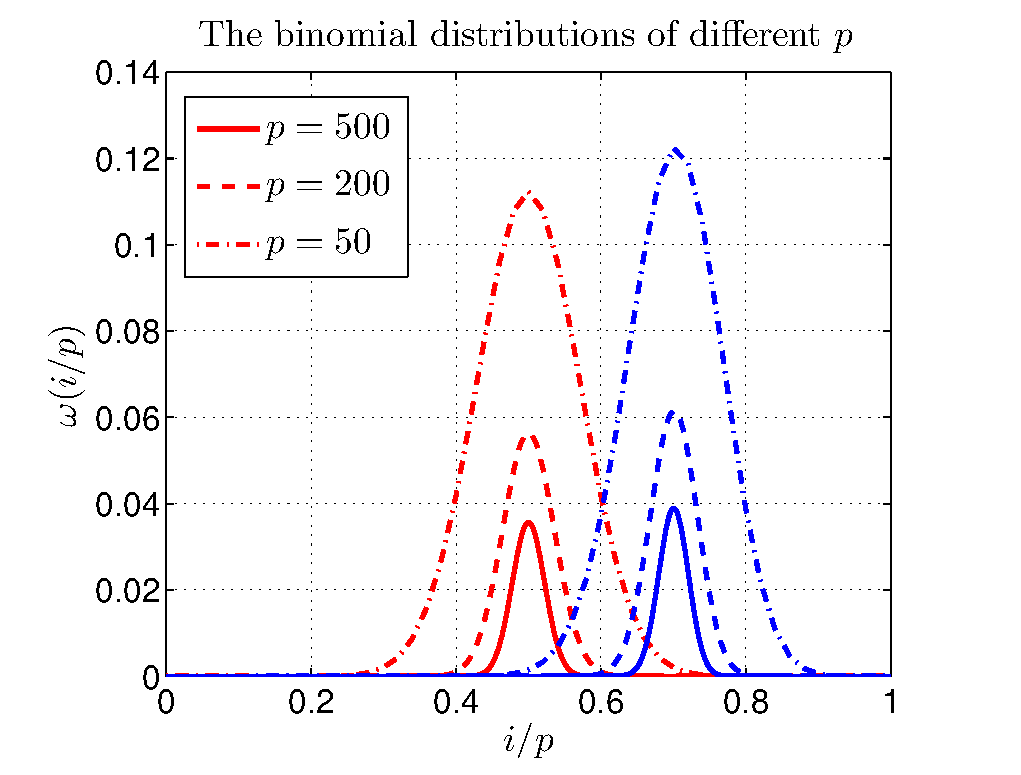
\includegraphics[width=0.5\textwidth]{deltaMexample1a}}
            {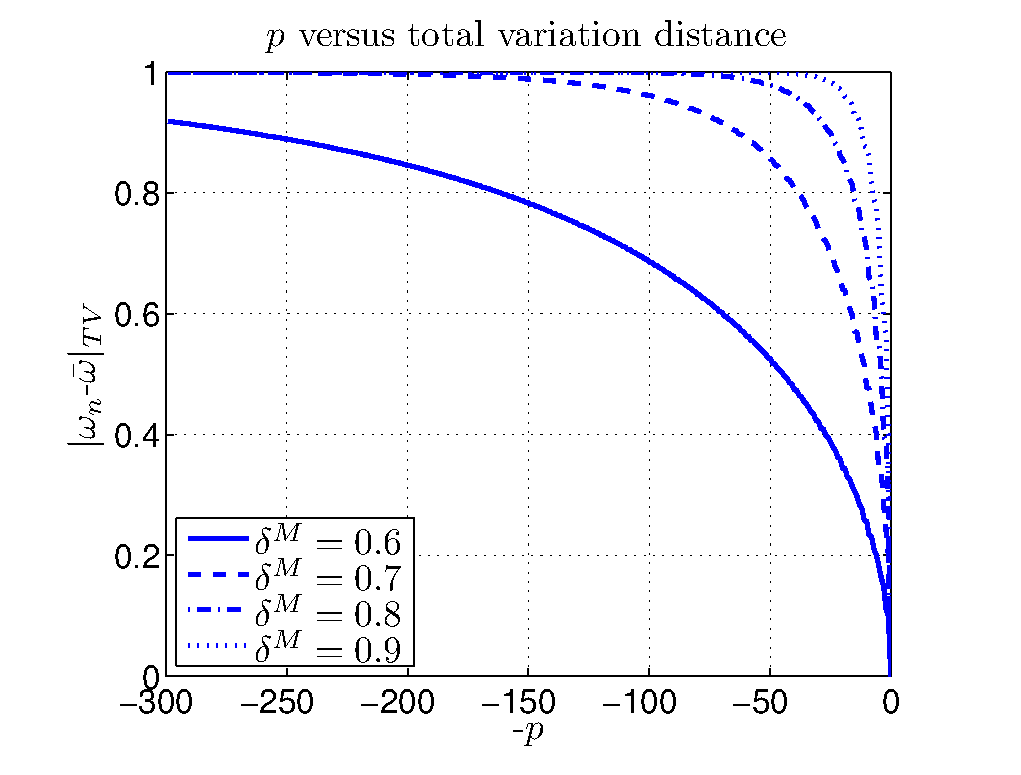
\includegraphics[width=0.5\textwidth]{deltaMexample1b}}}
\caption{\label{deltaMexample1}The left figure shows how one can evaluate
$|\omega^0-\bar{\omega}|_{TV}$, where $\omega^0$ has the form in equation (\ref{constantomega0}),
by finding the overlap area of two binomial distributions centered at $p\delta_\star^a$ and $p/2$.
When $p$ is large, the overlap area gets smaller. The right figure shows how
$|\omega^0-\bar{\omega}|_{TV}$ changes with $p$ for different $\delta_\star$'s. Since evolving
the distribution (\ref{constantomega0}) is equivalent to change $p$, this set of trajectories can
be also interpreted as $|\omega^k-\bar{\omega}|_{TV}$ for $k=300-p$}.
\end{figure}

\end{example}
From the above example, we can give the following theorem.
\begin{theorem}
For a $1$-D map $S:\Lambda \to \Lambda$ having symbolic dynamics, the family \\$(\Omega,\bar{\omega},(\omega^k_n)_{k=0,1,\ldots})_{n=1,2,\ldots}$ presents a total variation-cutoff in the relaxed sense, where
\begin{equation*} 
 \psi(\omega^0_n) =  \{.\underbrace{\delta_\star \delta_\star \cdots \delta_\star}_{n}\frac{1}{2}\frac{1}{2}\cdots\} 
\end{equation*}
for $\omega^0_n\in\bar{\Omega}$ and $0 \le \delta_\star \le 1$. 
\end{theorem}
\begin{proof}
Let $t_n = n$, when $k_n>(1+\epsilon)n$, $|\omega^k_n-\bar{\omega}|_{TV}=0$. When $k_n<(1-\epsilon)n$, $n-k_n>\epsilon n$, and 
\begin{align*}
      |\omega_n^{k_n}-\bar{\omega}|_{TV} &   = |\omega_n^{n-{(n-{k_n})}}-\bar{\omega}|_{TV} \\
                                         & \ge |\omega_n^{n-{\lceil\epsilon n \rceil}}-\bar{\omega}|_{TV}\\
                                         &   = |\omega_p^{{p-{\lceil\epsilon n \rceil}}}-\bar{\omega}|_{TV}  \text{ for any } p\ge n \\
                                         &\to 1 \text{ when } n \to \infty.
\end{align*}
\end{proof}

Theorem \ref{tentmapcutoff} is a special case of the above theorem with $\delta_\star = 1$. 



%%%%%%%%%%%%%%%%%%%%%%%%%%%%%%%%%%%%%%%%%%%%%%%%%%%%%%%%%%%%%%%%%%%%%%%%%%%%%%%%%%
\begin{example}
Suppose $\omega^0$ has stochastic symbol sequence as follows:
  \begin{eqnarray}
  \label{expw0}
   \psi(\omega^0) =  \{.\delta_0 \delta_1 \delta_2 \cdots\},
  \end{eqnarray}
where $\delta_i = \frac{1}{2} + \epsilon r^i$, $\epsilon \in [0,1/2]$ and $r\in [0,1]$. The reason we choose it to decay exponentially is that we can use the upper bound theorem with fixed $p$. Here the area under $\delta$ and above $\frac{1}{2}$ can be calculated by the sum of a geometric series. Let $(\delta^M_\star)^k = \delta_k$; then
  \begin{eqnarray}
   \frac{M_k}{2} = \frac{\delta_k}{1-r}.
  \end{eqnarray}
Hence choose $p = \lfloor \frac{1}{1-r} \rfloor $ for the upper bound theorem. $p$ is a constant so the analysis is easier (as we see in the previous example, $p$ affects the TV). We use the same $p$ for the lower bound theorem, so $(\delta^m_\star)^k = r^p(\delta_{k}-\frac{1}{2}) $. From the upper and lower bound theorems, the total variation distance to stationary at iteration $k$ can be bounded by
  \begin{eqnarray}
  \label{omegakbound}
    |\psi^{-1}((\delta^m)^k)-\bar{\omega}|_{TV} <|\omega^k-\bar{\omega}|_{TV}<|\psi^{-1}((\delta^M)^k)-\bar{\omega}|_{TV},
  \end{eqnarray}
where
  \begin{eqnarray}
  \label{defdeltamM}
   (\delta^m)^k = \{.\underbrace{(\delta^m_\star)^k (\delta^m_\star)^k \cdots (\delta^m_\star)^k}_{p}\frac{1}{2}\frac{1}{2}\cdots\}, \nonumber\\
   (\delta^M)^k = \{.\underbrace{(\delta^M_\star)^k (\delta^M_\star)^k \cdots (\delta^M_\star)^k}_{p}\frac{1}{2}\frac{1}{2}\cdots\}.
  \end{eqnarray}

\begin{figure}
\centerline{{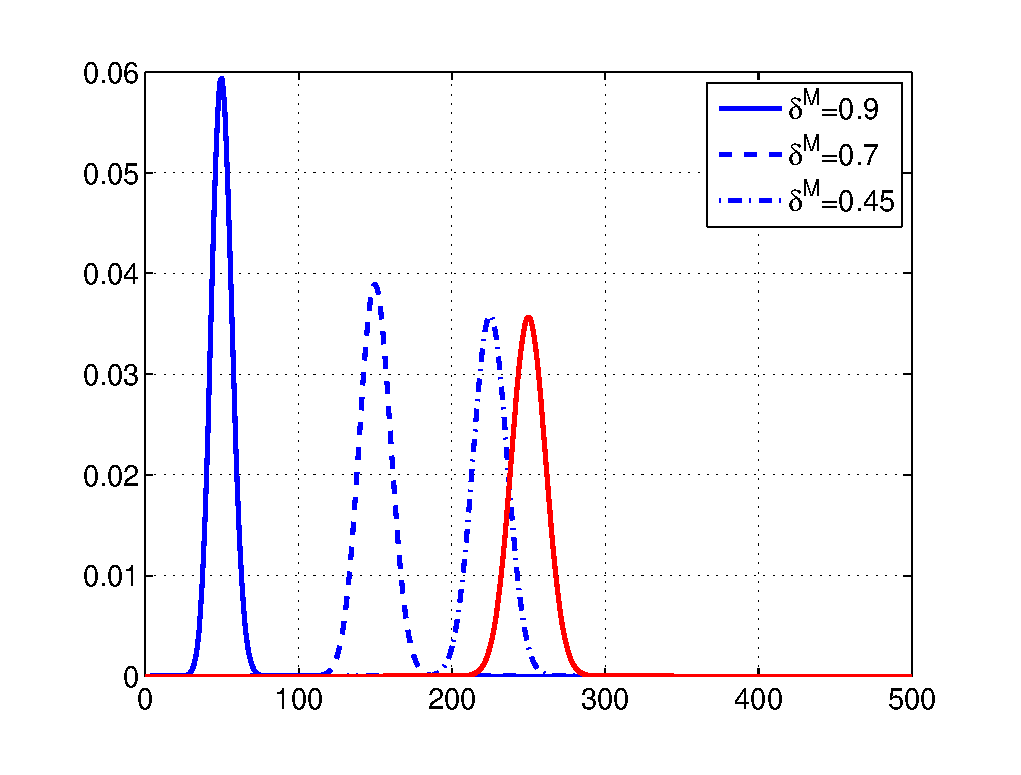
\includegraphics[width=0.5\textwidth]{deltaMexample2a}}
            {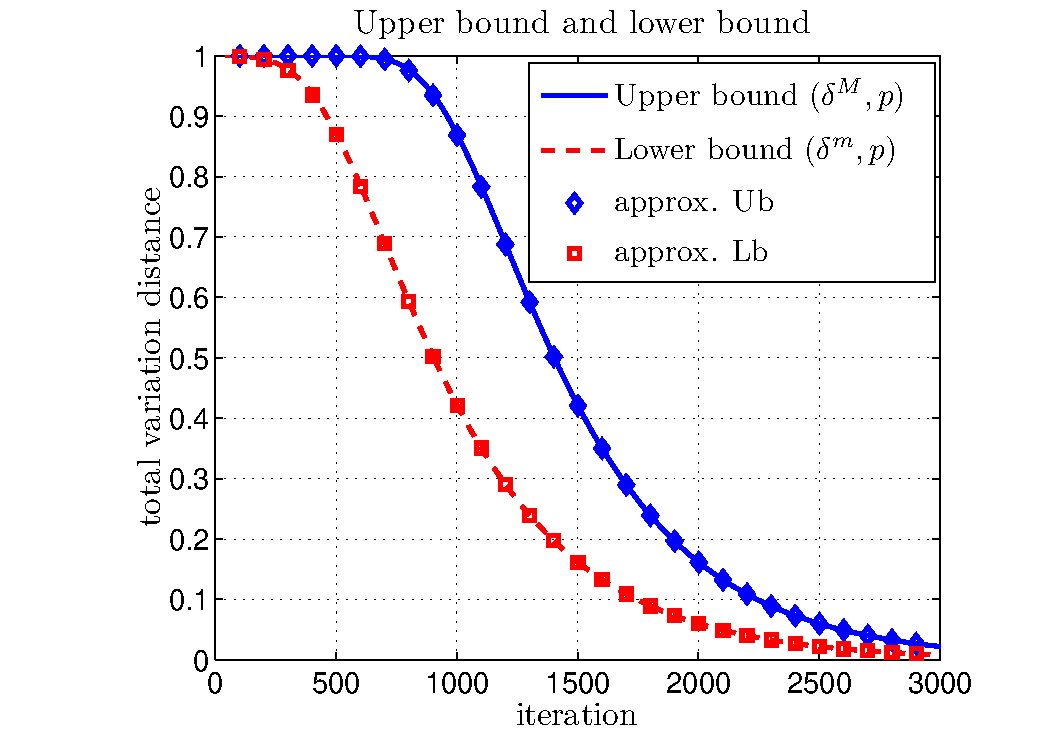
\includegraphics[width=0.5\textwidth]{deltaMexample2b}}}
\caption{\label{deltaMexample2}The left figure shows how one can evaluate the lower and upper
bounds of $|\omega^k-\bar{\omega}|_{TV}$, where $\omega^0$ has the form in equation (\ref{expw0}),
by finding the overlap area of two binomial distributions centered at
$p\delta_k=\frac{1}{2}+\epsilon r^k$ and $p/2$. In the right figure the upper bound and the lower
bound of $|\omega^k-\bar{\omega}|_{TV}$ by Theorems \ref{theoremub2} and \ref{theoremlb} are plotted,
as well as their approximations by Theorem \ref{theoremapproxlb}.}
\end{figure}
This is valid for each $k$. Similar to Example \ref{example:constantoega0}, we can plot the upper and lower bounds in a reduced space to see the movement of a binomial distribution. The left plot of Figure \ref{deltaMexample2} shows how the upper bound distribution moves toward the binomial distribution
centered at $p/2$ when $k$ increases, and then the TVs of upper bound and lower bound versus iteration plot is given
in the right plot of Figure \ref{deltaMexample2} for $\delta_0= 1$ and $r=0.998$.
Again, from the change of the overlap area of the left plot, it is not hard to understand how the concave shape is formed in the right plot.  

We need to stress here that to find the actual $|\omega^k-\bar{\omega}|_{TV}$ trajectory is impossible because one needs to evaluate (\ref{infiniteTV}) for each $\omega^k$. Even just to find an approximation of it using (\ref{finiteTV}), the computation cost is extremely large. This demonstrates the value of the upper and lower bound theorems. However, even so, we do not get much insight on how the bounds evolve because these two theorems give bounds based on the incomplete beta function. Hence here we would like to apply Theorem \ref{theoremapproxlb} regardless of its condition ($p \to \infty$ and $\delta_\star \to 1$). It should give us a pair of approximate upper and lower bounds,
\begin{eqnarray}
\label{expub}
|\omega^k -\bar{\omega}|_{TV}  &\stackrel{approx.}{\le}  &  \erf\left( \sqrt{\frac{p}{2}}\left((\delta_{\star}^M)^k-\frac{1}{2}\right)\right) \nonumber \\
                               & = &     \erf\left( \sqrt{\frac{1}{2(1-r)}} \epsilon^0r^k \right),
\end{eqnarray}
and
\begin{eqnarray}
\label{explb}
|\omega^k -\bar{\omega}|_{TV}  &\stackrel{approx.}{\ge} & \erf\left( \sqrt{\frac{1}{2(1-r)}} \epsilon^0 r^{\frac{1}{1-r}}r^k \right)  \nonumber \\
                               & = &  \erf\left( \sqrt{\frac{1}{2(1-r)}} \epsilon^0 e^{-1} r^k \right).
\end{eqnarray}
The approximated upper and lower bounds are plotted in the right of Figure \ref{deltaMexample2}, too. They are almost identical to the actual bounds.
Both (\ref{explb}) and (\ref{expub}) show the normal shapes, just like we see in example 1. Since
$(\delta_{\star}^M)^k-\frac{1}{2} = \epsilon^0 r^k$ decays exponentially (with factor $r$) to $0$, the trajectory
does not look like the error function itself. Instead, it has a sharper change before cutoff
happens and gets milder after it.
\end{example}
%%%%%%%%%%%%%%%%%%%%%%%%%%%%%%%%%%%%%%%%%%%%%%%%%%%%%%%%%%%%%%%%%%%%%%%%%%%%%%%%%%%%

The above two examples show the impact of $p$ and $\delta_{\star}^M$, which relate to the sum of
the stochastic symbol sequence and its largest entry. To summarize, the TV of the current distribution to the invariant distribution can be characterized by its upper and lower bounds, which correspond to $|\psi( (\delta^m)^k )^{-1}-\bar{\omega}|_{TV}$ and $|\psi( (\delta^M)^k )^{-1}-\bar{\omega}|_{TV}$. They
can be evaluated (and also approximated) and then the shape of $|\omega-\bar{\omega}|_{TV}$ is determined.
% which
%centered at $p\delta_{\star}^M$ (resp. $p\delta_{\star}^m$) and $p/2$. And so their TV can be bounded by $p$ and $\delta_{\star}^M$ (resp. $\delta_{\star}^m$). Isolating the
%change of $p$ or $\delta_{\star}^M$($\delta_{\star}^m$), the trajectory can be shown as the right
%plot of figure \ref{deltaMexample1} and the right plot of figure \ref{deltaMexample2}.



\subsection{Create cutoffs}
We have shown that an initial distribution like (\ref{expw0}) evolved by $P_S$ can have very similar $|\omega^k-\bar{\omega}|_{TV}$ trajectory to what one sees in a cutoff phenomenon. Now we want to take a further step to show that we can generate a set of initial disitributions $\omega_n$, which are a function of $n$, such that $\nu_n^k = |\omega_n^k-\bar{\omega}|_{TV}$ actually has the shape of (\ref{rdwalkshape}) when $n$ goes to infinity. We give the following theorem.
%%%%%%%%%%%%%%%%%%%%%%%%%%%%%%%%%%%%%%%%%%%%%%%%%%%%%%%%%%%%%%%%%%%%%%%%%%%%%%%%%%%%%
\begin{theorem}
Let $\omega_n^0 \in \bar{\Omega}$ have stochastic symbol sequence
 \begin{eqnarray}
    \psi(\omega^0_n) =  \{.\delta_0 \delta_1 \delta_2 \cdots\},
 \end{eqnarray}
where $\delta_i = \min\{\frac{1}{2}+\epsilon_n r_n^i,1\}$, and
 \begin{align}
 \begin{split}
          r_n &= e^{-\frac{2}{n}}.\\
          \epsilon_n &= \sqrt{\frac{n(1-r_n)}{4}},
 \end{split}
 \end{align}
The family $(\Omega,\bar{\omega},(\omega^k_n)_{k=0,1,\ldots})_{n=1,2,\ldots}$ presents a total variation-cutoff. In fact, 
Let $k = \frac{1}{4}n\log{n}+cn $; then for fixed $c\in \mathbb{R}$ as $n\to \infty$,
\begin{eqnarray}
\label{erfbound}
 %|\omega^k_n - \bar{\omega} |_{TV} \sim \erf \left(\frac{e^{-2c}}{\sqrt{8}}\right)
          \erf \left(\frac{e^{-2c-1}}{\sqrt{8}}\right)\le  |\omega^k_n - \bar{\omega} |_{TV} \le \erf \left(\frac{e^{-2c}}{\sqrt{8}}\right).
\end{eqnarray}
\end{theorem}

\begin{proof} From example 3, $|\omega^k_n - \bar{\omega}|_{TV}$ is bounded by (\ref{omegakbound}). When $n \to \infty$, $\epsilon_n$ goes to $\sqrt{\frac{1}{2}}$ and $r_n$ goes to $1$. Letting $k> \frac{-\log(2\epsilon_n)}{r_n}$ so that $\epsilon_n r_n^k<1/2$, and using the results of (\ref{expub}) and (\ref{explb}), we have
\begin{eqnarray}
                \erf\left( \sqrt{\frac{1}{2(1-r_n)}} \epsilon_n e^{-1} r_n^k \right)
            \le |\omega^k_n - \bar{\omega}|_{TV}
            \le \erf\left( \sqrt{\frac{1}{2(1-r_n)}} \epsilon_nr_n^k \right).
\end{eqnarray}
Now these bounds are not approximations because the conditions of Theorem \ref{theoremapproxlb} are satisfied. 
Substituting the expresstion $\epsilon_n$ and $r_n$ into above inequality gives
\begin{eqnarray}
                \erf\left(\sqrt{\frac{n}{8}}e^{-\frac{2k}{n}-1}  \right)
            \le |\omega^k_n - \bar{\omega}|_{TV}
            \le  \erf\left(\sqrt{\frac{n}{8}}e^{-\frac{2k}{n}}  \right),
\end{eqnarray}
%Thus we have
%\begin{eqnarray}
  %     |\omega^k_n - \bar{\omega} |_{TV} \sim \erf\left(\sqrt{\frac{n}{8}}e^{-\frac{2k}{n}}  \right)
%\end{eqnarray}
Letting $k = \frac{1}{4}n\log{n}+cn $ for $c\in \mathbb{R}$, and substituting into the above expression, we get the desired result (\ref{erfbound}), and hence it presents a cutoff.
\end{proof}

%%%%%%%%%%%%%%%%%%%%%%%%%%%%%%%%%%%%%%%%%%%%%%%%%%%%%%%%%%%%%%%%%%%%%%%%%%%%%%%%%%%%%%

The key idea of the above theorem is that we know for a pair of $(\epsilon,r)$, the stochastic symbol sequence with $\delta_i = \frac{1}{2}+\epsilon r^i$ has a normal shape cutoff. Hence we equate the coefficients to find $(\epsilon_n,r_n)$ as functions of $n$ that have the same $|\omega^k_n - \bar{\omega} |_{TV}$ as the random walk on a $n$-dimensional hypercube problem. In this case the $\epsilon_n$ we find is larger than $1/2$ when $n>1$, which is prohibited in the stochastic symbol sequence ($\delta_0>1$). However, we set $\delta^i=1$ for $i<\frac{-\log(2\epsilon_n)}{r_n}$ and then when $k> \frac{-\log(2\epsilon_n)}{r_n}$, the remaining sequence is exponential and Theorem \ref{theoremapproxlb} is applicable again.

Following the same rule, we can reproduce any cutoff with normal shape in relaxed sense by a family $\{\Omega,\bar{\omega},(\omega_n^k)_{k=0,1,\ldots}\}_{n=0,1,\ldots}$, where $\omega_n^{k+1} = P_S(\omega_n^k)$, and $P_S$ is the Perron-Frobenius of map $S:\Lambda \to \Lambda$, which has symbolic dynamics.


%%%%%%%%%%%%%%%%%%%%%%%%%%%%%%%%%%%%%%%%%%%%%%%%
\subsection{What causes cutoffs?}
%%%%%%%%%%%%%%%%%%%%%%%%%%%%%%%%%%%%%%%%%%%%%%%%
As we have mentioned before, the analysis and proof of cutoffs are usually very hard, but to understand what causes cutoffs can be quite easy and we discuss it here to further explain the relation between the cutoff of finite Markov Chains and chaotic map mixing. Let us focus on the total variation-cutoff with normal shape. We claim that if the process is composed of many (almost) independent small processes, then it has the key factor to present a cutoff. To explain this, again we use the random walk on an $n$-dimensional hypercube as the example. Let $I=\{0,1\}$; the coordinate of the particle can be represented as a vector in $I^n$. For instance, the point starting at the origin is
\begin{eqnarray*}
 x^0 = (0,0,\ldots,0).
\end{eqnarray*}
Each of the coordinates equals zero with probability $1$. At each iteration, the particle can stay fixed or choose one of the coordinates randomly. For this chosen coordinate, if it is $0$, it becomes $1$ and vice versa. Under this big process with $n$ coordinates and $2^n$ states, we can discuss $n$ much smaller random processes: the value of each coordinate. All of these small processes are not independent of each other. For example, at iteration $1$, suppose we know that the first coordinate is $1$; then we immediately know all of the other coordinates are zeros. 
So even though all of these small processes are identical and easy to analyze, to calculate the probability of the $2^n$ states by the joint probability of the small processes is still not possible. Nonetheless, a very important fact is: they become almost independent after just several iterations. This is also easy to imagine: suppose $n = 1000$ and $k = 10$; knowing that the first coordinate is $1$ is almost not helpful to know the value of any other coordinates. The tendency that these small processes have to become independent of each other is so strong that even if we just assume they are independent in the beginning, and calculate $\omega_n^k$ by the joint probability of these independent small processes, we get a very good approximation of the actual process. This simplification corresponds to the continuous-time random walk on a hypercube problem \cite{Diaconis1990}. The analysis of this problem is much easier than the original problem and it presents the same cutoff. Therefore, we can conclude that even if the original process is very complicated, the almost independence of the small processes is the key for the whole process to present a cutoff. 

Then how does this almost independence fit into the chaotic map evolution? Remember that the probability space we discuss is $\bar{\Omega}$, and from Lemma \ref{lemma:independency}, when a point $x$ with probability distribution $\omega \in \bar{\Omega}$ is evolved by the chaotic map with symbolic dynamics, $\phi(x^k)_i$ and $\phi(x^k)_j$ are independent of each other for all $k$ and $i\neq j$. So this process looks like it is composed of an infinite number of independent small processes. Thus we can design the exponential type stochastic symbol sequence to make all these small processes behave like the process we see in one coordinate of the hypercube and achieve similar TV trajectories. It is purely the special property of $\omega \in \bar{\Omega}$ for chaotic maps with symbolic dynamics that makes this possible. This clearly explains why we observe cutoffs in chaotic map evolution.  

 

%%%%%%%%%%%%%%%%%%%%%%%%%%%%%%%%%%%%%%%%%%%%%%%%
%\subsection{When $\omega \notin \bar{\Omega}$}
%%%%%%%%%%%%%%%%%%%%%%%%%%%%%%%%%%%%%%%%%%%%%%%%

%The above results are only applicable when $\omega \in \bar{\Omega}$, and is quite restrictive. An easy extension can be made for all $\omega \in \Omega$ and are ``close'' to $\bar{\Omega}$ in total variation distance. Given $\omega^0 \in \Omega $, suppose we can find an $\tilde{\omega}^0\in \bar{\Omega} $ such that $|\omega^0- \tilde{\omega}^0|_{TV}$ is small, then use triangular inequality, for any $k \ge 0$
%\begin{eqnarray}
%     \left| |\tilde{\omega}^k-\bar{\omega} |_{TV}  -  |\omega^k-\tilde{\omega}^k|_{TV}\right|
%     \le |\omega^k-\bar{\omega}|_{TV}
%     \le |\tilde{\omega}^k-\bar{\omega}|_{TV} + |\omega^k-\tilde{\omega}^k|_{TV}
%\end{eqnarray}
%Total variation distance is non-increasing, thus $|\omega^k-\tilde{\omega}^k|_{TV} \le |\omega^0-\tilde{\omega}^0|_{TV} $. Let the upper and lower bounds obtained by theorem \ref{theoremub} and \ref{theoremlb} for $|\tilde{\omega}^k-\bar{\omega} |_{TV}$ be $b_l^k$ and $b_u^k$, and let $|\omega^0-\tilde{\omega}^0|_{TV} = b^0$, we have
%\begin{eqnarray}
%     |b_l^k-b^0| \le |\omega^k-\bar{\omega}|_{TV}  \le b_u^k+b^0
%\end{eqnarray}
%How do we find $\tilde{\omega}^0$ such that $|\omega^0- \tilde{\omega}^0|_{TV}$ is minimized so that the bound is tighter? The easiest way is letting $\tilde{\omega}^0 = \psi(\omega^0) $. This may not be the best fitting of $\omega^0$, however, it is believed that if $\psi(\omega^0)$ is not a good fitting of $\omega^0$, there is not much space to improved by finding another $\tilde{\omega}^0$. Again, we want to stress that the upper and lower bounds are not practically useful, but they do characterize the behavior of the convergence trajectory for a set of $\omega^0$.


